\chapter{Cardinality: Measuring the Infinite}

\section{The Problem of Infinite Size}

\begin{intuition}
For finite sets, counting is straightforward: $\{a, b, c\}$ has size 3.

But what does it mean for $\mathbb{N}$ and $\mathbb{Z}$ to have the ``same size''?

\begin{itemize}
    \item Intuition says $\mathbb{Z}$ is ``twice as large'' (it has negatives too)
    \item But we can pair them perfectly: $0 \leftrightarrow 0$, $1 \leftrightarrow 1$, $2 \leftrightarrow -1$, $3 \leftrightarrow 2$, $4 \leftrightarrow -2$, \dots
\end{itemize}

Georg Cantor (1874) revolutionized mathematics by showing:
\begin{enumerate}
    \item Bijections measure size, even for infinite sets
    \item Not all infinities are equal
    \item There's an infinite hierarchy of infinities
\end{enumerate}
\end{intuition}

\begin{historicalnote}
\textbf{Cantor's Journey (1845-1918)}

Cantor's set theory was initially rejected as ``dangerous'' mathematical heresy:
\begin{itemize}
    \item \textbf{Kronecker} called it ``mathematical insanity''
    \item \textbf{Poincaré} called it a ``disease from which mathematics would recover''
    \item Cantor suffered depression and was institutionalized multiple times
\end{itemize}

But today, Cantor's ideas are foundational:
\begin{itemize}
    \item \textbf{Hilbert} (1900): ``No one shall expel us from the paradise that Cantor has created''
    \item \textbf{Bertrand Russell}: ``One of the greatest achievements of the human intellect''
\end{itemize}

The diagonal argument is now considered one of the most beautiful proofs in mathematics.
\end{historicalnote}

\section{Cardinality: The Formal Definition}

\begin{definition}[Cardinality]
Two sets $A$ and $B$ have the same \textbf{cardinality} (written $|A| = |B|$ or $A \approx B$) if there exists a bijection $f: A \to B$.

We say:
\begin{itemize}
    \item $|A| \leq |B|$ if there exists an injection $f: A \to B$
    \item $|A| < |B|$ if $|A| \leq |B|$ but $|A| \neq |B|$
\end{itemize}
\end{definition}

\begin{keyidea}
Cardinality abstracts the notion of ``counting'' to infinite sets:

\textbf{For finite sets}: $|A| = n$ means we can list elements as $a_1, a_2, \ldots, a_n$

\textbf{For infinite sets}: $|A| = |B|$ means we can pair elements perfectly with no leftovers

Bijections are the \textit{only} way to rigorously compare sizes of infinite sets.
\end{keyidea}

\begin{center}
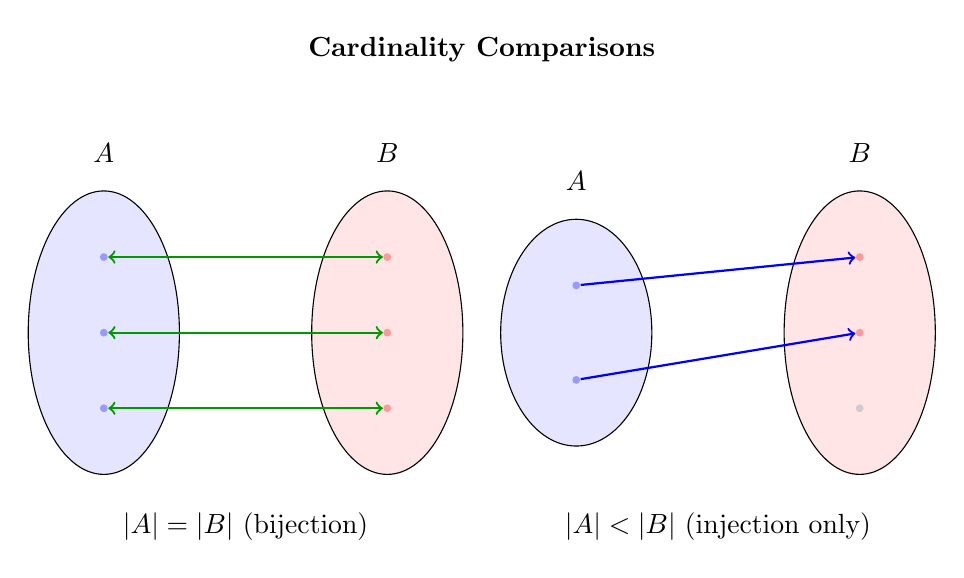
\begin{tikzpicture}[scale=1.2]
    \node at (4, 5) {\textbf{Cardinality Comparisons}};
    
    % |A| = |B|
    \begin{scope}[shift={(0,2)}]
        \draw[fill=blue!10] (0,0) ellipse (0.8cm and 1.5cm);
        \draw[fill=red!10] (3,0) ellipse (0.8cm and 1.5cm);
        \node[above] at (0,1.7) {$A$};
        \node[above] at (3,1.7) {$B$};
        
        \node[circle, fill=blue!40, inner sep=1pt] (a1) at (0,0.8) {};
        \node[circle, fill=blue!40, inner sep=1pt] (a2) at (0,0) {};
        \node[circle, fill=blue!40, inner sep=1pt] (a3) at (0,-0.8) {};
        
        \node[circle, fill=red!40, inner sep=1pt] (b1) at (3,0.8) {};
        \node[circle, fill=red!40, inner sep=1pt] (b2) at (3,0) {};
        \node[circle, fill=red!40, inner sep=1pt] (b3) at (3,-0.8) {};
        
        \draw[<->, thick, green!60!black] (a1) -- (b1);
        \draw[<->, thick, green!60!black] (a2) -- (b2);
        \draw[<->, thick, green!60!black] (a3) -- (b3);
        
        \node[below] at (1.5, -1.8) {$|A| = |B|$ (bijection)};
    \end{scope}
    
    % |A| < |B|
    \begin{scope}[shift={(5,2)}]
        \draw[fill=blue!10] (0,0) ellipse (0.8cm and 1.2cm);
        \draw[fill=red!10] (3,0) ellipse (0.8cm and 1.5cm);
        \node[above] at (0,1.4) {$A$};
        \node[above] at (3,1.7) {$B$};
        
        \node[circle, fill=blue!40, inner sep=1pt] (a1) at (0,0.5) {};
        \node[circle, fill=blue!40, inner sep=1pt] (a2) at (0,-0.5) {};
        
        \node[circle, fill=red!40, inner sep=1pt] (b1) at (3,0.8) {};
        \node[circle, fill=red!40, inner sep=1pt] (b2) at (3,0) {};
        \node[circle, fill=gray!40, inner sep=1pt] (b3) at (3,-0.8) {};
        
        \draw[->, thick, blue] (a1) -- (b1);
        \draw[->, thick, blue] (a2) -- (b2);
        
        \node[below] at (1.5, -1.8) {$|A| < |B|$ (injection only)};
    \end{scope}
\end{tikzpicture}
\end{center}

\begin{theorem}[Properties of Cardinality]
Cardinality satisfies:
\begin{enumerate}
    \item \textbf{Reflexivity}: $|A| = |A|$ (identity function)
    \item \textbf{Symmetry}: $|A| = |B| \implies |B| = |A|$ (inverse bijection)
    \item \textbf{Transitivity}: $(|A| = |B| \land |B| = |C|) \implies |A| = |C|$ (composition)
\end{enumerate}

Therefore, ``same cardinality'' is an equivalence relation on sets.
\end{theorem}

\begin{proof}
\textbf{Reflexivity}: The identity function $\text{id}_A: A \to A$ is a bijection. $\checkmark$

\textbf{Symmetry}: If $f: A \to B$ is a bijection, then $f^{-1}: B \to A$ exists and is a bijection. $\checkmark$

\textbf{Transitivity}: If $f: A \to B$ and $g: B \to C$ are bijections, then $g \circ f: A \to C$ is a bijection. $\checkmark$
\end{proof}

\section{Countable Sets: The Smallest Infinity}

\begin{definition}[Countable Sets]
A set $A$ is:
\begin{itemize}
    \item \textbf{Finite} if $|A| = n$ for some $n \in \mathbb{N}$ (including empty set)
    \item \textbf{Countably infinite} if $|A| = |\mathbb{N}|$ (bijection with natural numbers)
    \item \textbf{Countable} if it is finite or countably infinite
    \item \textbf{Uncountable} if it is not countable
\end{itemize}

The cardinality of $\mathbb{N}$ is denoted $\aleph_0$ (aleph-null, read ``aleph-naught'').
\end{definition}

\begin{keyidea}
A set is countably infinite if we can \textbf{list} its elements:
\[A = \{a_1, a_2, a_3, \ldots\}\]

The bijection $f: \mathbb{N} \to A$ is given by $f(n) = a_n$.

``Countable'' means ``no bigger than $\mathbb{N}$''---we can count the elements (even if it takes forever).
\end{keyidea}

\subsection{The Integers are Countable}

\begin{theorem}
$|\mathbb{Z}| = |\mathbb{N}| = \aleph_0$
\end{theorem}

\begin{proof}
We construct an explicit bijection $f: \mathbb{N} \to \mathbb{Z}$:

\[f(n) = \begin{cases}
0 & \text{if } n = 0 \\
\frac{n}{2} & \text{if } n > 0 \text{ and } n \text{ is even} \\
-\frac{n+1}{2} & \text{if } n > 0 \text{ and } n \text{ is odd}
\end{cases}\]

Alternatively (starting from 1):
\[g(n) = \begin{cases}
\frac{n}{2} & \text{if } n \text{ is even} \\
-\frac{n-1}{2} & \text{if } n \text{ is odd}
\end{cases}\]

This produces the sequence:
\begin{align*}
g(1) &= 0 \\
g(2) &= 1 \\
g(3) &= -1 \\
g(4) &= 2 \\
g(5) &= -2 \\
g(6) &= 3 \\
&\vdots
\end{align*}

\textbf{Injectivity}: If $g(m) = g(n)$, we must show $m = n$.

\textit{Case 1}: Both $m, n$ even. Then $\frac{m}{2} = \frac{n}{2}$, so $m = n$. $\checkmark$

\textit{Case 2}: Both $m, n$ odd. Then $-\frac{m-1}{2} = -\frac{n-1}{2}$, so $m-1 = n-1$, thus $m = n$. $\checkmark$

\textit{Case 3}: One even, one odd. Then $g(m) > 0$ but $g(n) \leq 0$ (or vice versa), so $g(m) \neq g(n)$. $\checkmark$

\textbf{Surjectivity}: Let $k \in \mathbb{Z}$.

\textit{If $k > 0$}: Let $n = 2k$ (even). Then $g(n) = \frac{2k}{2} = k$. $\checkmark$

\textit{If $k \leq 0$}: Let $n = -2k + 1$ (odd). Then $g(n) = -\frac{(-2k+1)-1}{2} = -\frac{-2k}{2} = k$. $\checkmark$

Therefore $g$ is a bijection, so $|\mathbb{Z}| = |\mathbb{N}|$.
\end{proof}

\begin{center}
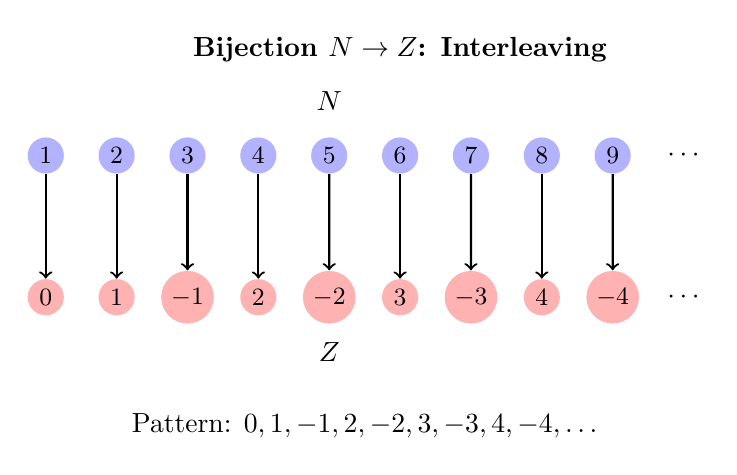
\begin{tikzpicture}[scale=0.9]
    \node at (5, 3.5) {\textbf{Bijection $\mathbb{N} \to \mathbb{Z}$: Interleaving}};
    
    % Natural numbers
    \foreach \x/\n in {0/1, 1/2, 2/3, 3/4, 4/5, 5/6, 6/7, 7/8, 8/9} {
        \node[circle, fill=blue!30, inner sep=2pt] (n\x) at (\x, 2) {\small $\n$};
    }
    \node at (9, 2) {$\cdots$};
    \node[above] at (4, 2.5) {$\mathbb{N}$};
    
    % Integers
    \foreach \x/\z in {0/0, 1/1, 2/-1, 3/2, 4/-2, 5/3, 6/-3, 7/4, 8/-4} {
        \node[circle, fill=red!30, inner sep=2pt] (z\x) at (\x, 0) {\small $\z$};
    }
    \node at (9, 0) {$\cdots$};
    \node[below] at (4, -0.5) {$\mathbb{Z}$};
    
    % Arrows
    \foreach \x in {0,1,2,3,4,5,6,7,8} {
        \draw[->, thick] (n\x) -- (z\x);
    }
    
    \node[below] at (4.5, -1.5) {Pattern: $0, 1, -1, 2, -2, 3, -3, 4, -4, \ldots$};
\end{tikzpicture}
\end{center}

\begin{remark}
This is counterintuitive! $\mathbb{Z}$ appears to have ``twice as many'' elements (positive and negative), but bijections reveal they're the same size.

This is the beginning of Hilbert's Hotel: an infinite hotel with rooms numbered $1, 2, 3, \ldots$ can always fit more guests, even infinitely many more.
\end{remark}

\subsection{Cartesian Products of Countable Sets}

\begin{theorem}
$|\mathbb{N} \times \mathbb{N}| = |\mathbb{N}| = \aleph_0$
\end{theorem}

\begin{proof}
We need a bijection $f: \mathbb{N} \times \mathbb{N} \to \mathbb{N}$.

One explicit construction uses \textbf{Cantor's pairing function}:
\[f(m, n) = \frac{(m + n)(m + n + 1)}{2} + n\]

This is injective and surjective (proof omitted, but verifiable).

Alternatively, we can visualize pairs $(m, n)$ in a grid and traverse them diagonally:

\begin{center}
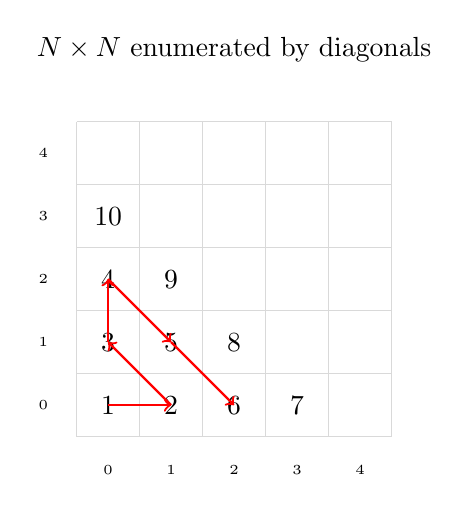
\begin{tikzpicture}[scale=0.8]
    \draw[step=1, gray!30] (0,0) grid (5,5);
    
    % Coordinates
    \foreach \x in {0,...,4} {
        \node[below] at (\x + 0.5, -0.3) {\tiny $\x$};
    }
    \foreach \y in {0,...,4} {
        \node[left] at (-0.3, \y + 0.5) {\tiny $\y$};
    }
    
    % Diagonal traversal
    \node at (0.5, 0.5) {1};
    \node at (1.5, 0.5) {2};
    \node at (0.5, 1.5) {3};
    \node at (0.5, 2.5) {4};
    \node at (1.5, 1.5) {5};
    \node at (2.5, 0.5) {6};
    \node at (3.5, 0.5) {7};
    \node at (2.5, 1.5) {8};
    \node at (1.5, 2.5) {9};
    \node at (0.5, 3.5) {10};
    
    \draw[->, thick, red] (0.5, 0.5) -- (1.5, 0.5);
    \draw[->, thick, red] (1.5, 0.5) -- (0.5, 1.5);
    \draw[->, thick, red] (0.5, 1.5) -- (0.5, 2.5);
    \draw[->, thick, red] (0.5, 2.5) -- (1.5, 1.5);
    \draw[->, thick, red] (1.5, 1.5) -- (2.5, 0.5);
    
    \node[above] at (2.5, 5.8) {$\mathbb{N} \times \mathbb{N}$ enumerated by diagonals};
\end{tikzpicture}
\end{center}

Follow the red path: we hit every pair $(m, n)$ eventually.

Therefore $|\mathbb{N} \times \mathbb{N}| = |\mathbb{N}|$.
\end{proof}

\begin{corollary}
If $A$ and $B$ are countable, then $A \times B$ is countable.
\end{corollary}

\begin{corollary}[Finite Products are Countable]
For any $k \in \mathbb{N}$, the Cartesian product $\mathbb{N}^k = \mathbb{N} \times \mathbb{N} \times \cdots \times \mathbb{N}$ ($k$ times) is countable.
\end{corollary}

\begin{proof}
By induction on $k$.

\textbf{Base case} ($k = 1$): $\mathbb{N}^1 = \mathbb{N}$ is countable by definition. $\checkmark$

\textbf{Inductive step}: Assume $\mathbb{N}^k$ is countable.

Then:
\[\mathbb{N}^{k+1} = \mathbb{N}^k \times \mathbb{N}\]

Since $\mathbb{N}^k$ and $\mathbb{N}$ are both countable (by inductive hypothesis and definition), the previous corollary shows their product $\mathbb{N}^{k+1}$ is countable. $\checkmark$

Therefore, by induction, $\mathbb{N}^k$ is countable for all $k \in \mathbb{N}$.
\end{proof}

\begin{remark}[Explicit Bijection $\mathbb{N}^k \to \mathbb{N}$]
While the inductive proof is elegant, one can also construct explicit bijections.

\textbf{For $\mathbb{N}^2 \to \mathbb{N}$:} Cantor's pairing function given above.

\textbf{For $\mathbb{N}^3 \to \mathbb{N}$:} Compose pairings:
\[\mathbb{N}^3 = \mathbb{N} \times \mathbb{N} \times \mathbb{N} \xrightarrow{f \times \text{id}} \mathbb{N} \times \mathbb{N} \xrightarrow{f} \mathbb{N}\]

where $f$ is Cantor's pairing function. Explicitly:
\[g(m, n, p) = f(f(m, n), p)\]

\textbf{For general $\mathbb{N}^k$:} Iterate Cantor's pairing function $k-1$ times:
\begin{align*}
h_k(n_1, n_2, \ldots, n_k) &= f(n_1, f(n_2, f(n_3, \ldots, f(n_{k-1}, n_k) \ldots)))
\end{align*}

Or, more computationally, use a \textbf{prime factorization encoding}:
\[h(n_1, n_2, \ldots, n_k) = 2^{n_1} \cdot 3^{n_2} \cdot 5^{n_3} \cdots p_k^{n_k}\]

where $p_1 = 2, p_2 = 3, p_3 = 5, \ldots$ are the first $k$ primes.

By the Fundamental Theorem of Arithmetic, each natural number has a unique prime factorization, so this map is injective. However, it is not surjective (not every natural number is a product of only the first $k$ primes), so this is an injection, not a bijection.

For a true bijection, Cantor's iterated pairing is simpler.
\end{remark}

\begin{theorem}[Countable Unions]\index{countable union}
\begin{enumerate}
    \item If $\{A_n : n \in \mathbb{N}\}$ is a countable collection of finite sets, then $\bigcup_{n=1}^\infty A_n$ is countable.
    
    \item If $\{A_n : n \in \mathbb{N}\}$ is a countable collection of countable sets, then $\bigcup_{n=1}^\infty A_n$ is countable.
\end{enumerate}
\end{theorem}

\begin{proof}
\textbf{(1) Countable union of finite sets:}

Let $A_1, A_2, A_3, \ldots$ be finite sets. We can assume they are pairwise disjoint (otherwise replace $A_n$ with $A_n \setminus (A_1 \cup \cdots \cup A_{n-1})$).

For each $n$, let $|A_n| = k_n$ (finite). Enumerate $A_n = \{a_{n,1}, a_{n,2}, \ldots, a_{n,k_n}\}$.

Consider the map $f: \bigcup_{n=1}^\infty A_n \to \mathbb{N} \times \mathbb{N}$ defined by:
\[f(a_{n,i}) = (n, i)\]

This is an injection (each element has a unique index pair). Since $\mathbb{N} \times \mathbb{N}$ is countable, and the union injects into it, the union is countable. $\checkmark$

\textbf{(2) Countable union of countable sets:}

Let $A_1, A_2, A_3, \ldots$ be countable sets. For each $n$, since $A_n$ is countable, there exists a bijection $g_n: \mathbb{N} \to A_n$ (or $g_n: \mathbb{N} \to A_n$ surjective if $A_n$ is finite, but we can pad with repetitions).

Define $f: \mathbb{N} \times \mathbb{N} \to \bigcup_{n=1}^\infty A_n$ by:
\[f(n, m) = g_n(m)\]

This is surjective: for any $a \in \bigcup A_n$, there exists $n$ such that $a \in A_n$. Since $g_n$ is a bijection (or surjection), there exists $m$ such that $g_n(m) = a$. Thus $f(n, m) = a$. $\checkmark$

Since there is a surjection from $\mathbb{N} \times \mathbb{N}$ (which is countable) onto $\bigcup A_n$, the union is countable. $\checkmark$
\end{proof}

\begin{remark}
This theorem is crucial for proving countability of algebraic numbers and other important sets. The key insight: arranging elements in a "grid" (indexed by two naturals) and using Cantor's diagonal argument allows us to enumerate the entire union.
\end{remark}

\subsection{The Rationals are Countable}

\begin{theorem}
$|\mathbb{Q}| = |\mathbb{N}| = \aleph_0$
\end{theorem}

\begin{proof}
We show $\mathbb{Q}^+$ (positive rationals) is countable; extending to all of $\mathbb{Q}$ is similar to the integer case.

Every positive rational can be written as $\frac{p}{q}$ with $p, q \in \mathbb{N}$, $q > 0$, $\gcd(p, q) = 1$ (reduced form).

Arrange fractions in a grid:
\begin{align*}
\text{Row 1: } & \frac{1}{1}, \frac{1}{2}, \frac{1}{3}, \frac{1}{4}, \ldots \\
\text{Row 2: } & \frac{2}{1}, \frac{2}{2}, \frac{2}{3}, \frac{2}{4}, \ldots \\
\text{Row 3: } & \frac{3}{1}, \frac{3}{2}, \frac{3}{3}, \frac{3}{4}, \ldots \\
&\vdots
\end{align*}

Traverse diagonally (as with $\mathbb{N} \times \mathbb{N}$), but \textbf{skip} any fraction already seen in reduced form:

\begin{center}
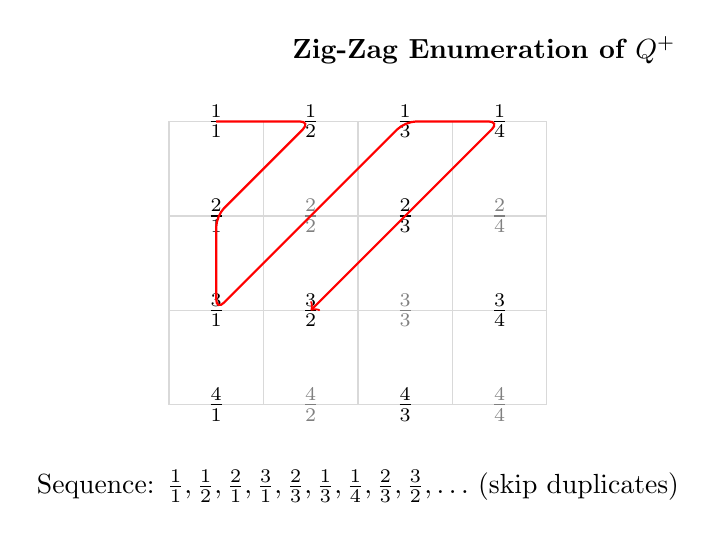
\begin{tikzpicture}[scale=1.0]
    \node at (4, 4.5) {\textbf{Zig-Zag Enumeration of $\mathbb{Q}^+$}};
    
    \draw[step=1.2, gray!30] (0,0) grid (4.8, 3.6);
    
    % Labels
    \node at (0.6, 3.6) {$\frac{1}{1}$};
    \node at (1.8, 3.6) {$\frac{1}{2}$};
    \node at (3.0, 3.6) {$\frac{1}{3}$};
    \node at (4.2, 3.6) {$\frac{1}{4}$};
    
    \node at (0.6, 2.4) {$\frac{2}{1}$};
    \node at (1.8, 2.4) {\color{gray} $\frac{2}{2}$};
    \node at (3.0, 2.4) {$\frac{2}{3}$};
    \node at (4.2, 2.4) {\color{gray} $\frac{2}{4}$};
    
    \node at (0.6, 1.2) {$\frac{3}{1}$};
    \node at (1.8, 1.2) {$\frac{3}{2}$};
    \node at (3.0, 1.2) {\color{gray} $\frac{3}{3}$};
    \node at (4.2, 1.2) {$\frac{3}{4}$};
    
    \node at (0.6, 0.0) {$\frac{4}{1}$};
    \node at (1.8, 0.0) {\color{gray} $\frac{4}{2}$};
    \node at (3.0, 0.0) {$\frac{4}{3}$};
    \node at (4.2, 0.0) {\color{gray} $\frac{4}{4}$};
    
    % Path
    \draw[->, thick, red, rounded corners] 
        (0.6, 3.6) -- (1.8, 3.6) -- (0.6, 2.4) -- (0.6, 1.2) -- (1.8, 2.4) -- (3.0, 3.6) -- (4.2, 3.6) -- (3.0, 2.4) -- (1.8, 1.2);
    
    \node[below] at (2.4, -0.7) {Sequence: $\frac{1}{1}, \frac{1}{2}, \frac{2}{1}, \frac{3}{1}, \frac{2}{3}, \frac{1}{3}, \frac{1}{4}, \frac{2}{3}, \frac{3}{2}, \ldots$ (skip duplicates)};
\end{tikzpicture}
\end{center}

This path hits every positive rational exactly once in lowest terms.

Therefore $|\mathbb{Q}^+| = |\mathbb{N}|$.

For all of $\mathbb{Q}$ (including negatives and zero), use the same interleaving trick as with $\mathbb{Z}$.

Therefore $|\mathbb{Q}| = |\mathbb{N}| = \aleph_0$.
\end{proof}

\begin{remark}
Stunning result: Between any two rationals, there are infinitely many more rationals (they're ``dense'' in $\mathbb{R}$), yet the rationals are the same size as the natural numbers!

But this is where Cantor's next result shatters intuition...
\end{remark}

\section{Cantor's Diagonal Argument: The Reals are Uncountable}

\begin{theorem}[Cantor's Diagonal Argument, 1891]\index{Cantor's diagonal argument}\index{diagonal argument}\index{uncountable sets}\index{real numbers!uncountability}
The interval $(0, 1)$ is uncountable:
\[|(0, 1)| > |\mathbb{N}|\]
\end{theorem}

\begin{proof}
We prove by \textbf{contradiction}.

Suppose $(0, 1)$ were countable. Then we could list all real numbers in $(0, 1)$:
\begin{align*}
n = 1: & \quad 0.d_{11} d_{12} d_{13} d_{14} d_{15} \ldots \\
n = 2: & \quad 0.d_{21} d_{22} d_{23} d_{24} d_{25} \ldots \\
n = 3: & \quad 0.d_{31} d_{32} d_{33} d_{34} d_{35} \ldots \\
n = 4: & \quad 0.d_{41} d_{42} d_{43} d_{44} d_{45} \ldots \\
&\vdots
\end{align*}

where $d_{ij} \in \{0, 1, 2, \ldots, 9\}$ are decimal digits.

We construct a number $X = 0.x_1 x_2 x_3 x_4 \ldots$ that is \textit{not} in this list:

Define $x_n$ by the rule:
\[x_n = \begin{cases}
1 & \text{if } d_{nn} \neq 1 \\
2 & \text{if } d_{nn} = 1
\end{cases}\]

(We ensure $x_n \neq 0, 9$ to avoid ambiguities like $0.999\ldots = 1.000\ldots$)

\textbf{Key observation}: $X$ differs from the $n$-th number in the list at the $n$-th decimal place:
\begin{itemize}
    \item $X$ differs from number 1 at digit 1
    \item $X$ differs from number 2 at digit 2
    \item $X$ differs from number 3 at digit 3
    \item \dots
\end{itemize}

Therefore $X$ is not equal to any number in the list.

But $X \in (0, 1)$ (it's a valid decimal between 0 and 1).

\textbf{Contradiction}: We assumed our list contained \textit{all} numbers in $(0, 1)$, but we just constructed a number not in the list.

Therefore, no such list exists. $(0, 1)$ is uncountable.
\end{proof}

\begin{center}
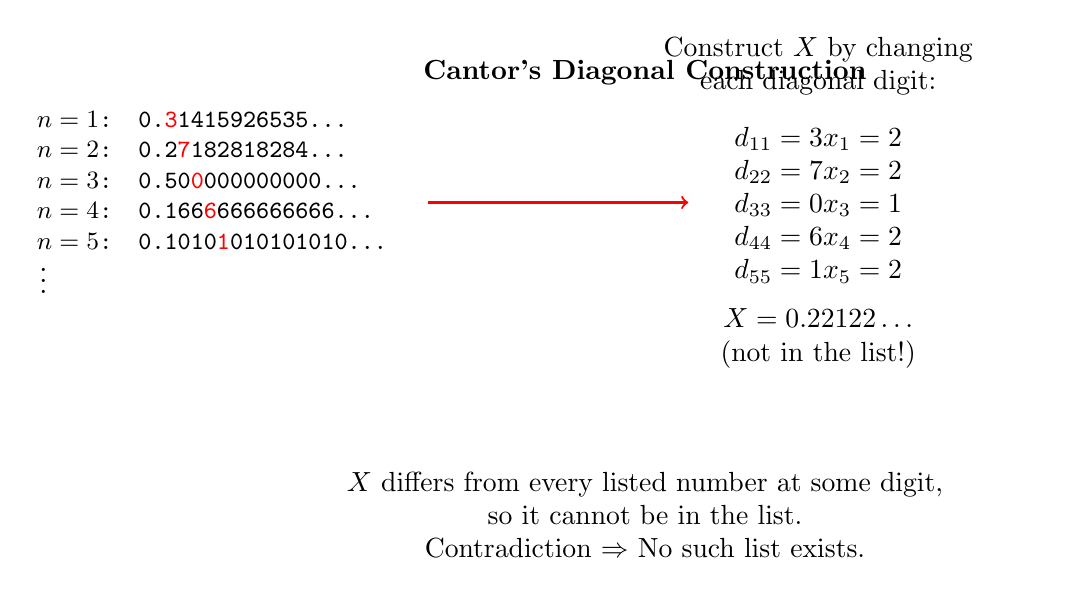
\begin{tikzpicture}[scale=1.1]
    \node at (5, 5) {\textbf{Cantor's Diagonal Construction}};
    
    \node[align=left, font=\ttfamily\small] at (0, 3.5) {
        $n=1$: 0.\textcolor{red}{3}1415926535... \\
        $n=2$: 0.2\textcolor{red}{7}182818284... \\
        $n=3$: 0.50\textcolor{red}{0}000000000... \\
        $n=4$: 0.166\textcolor{red}{6}666666666... \\
        $n=5$: 0.1010\textcolor{red}{1}010101010... \\
        $\vdots$
    };
    
    \node[align=center] at (7, 3.5) {
        Construct $X$ by changing \\
        each diagonal digit: \\[0.3cm]
        $d_{11} = 3 \implies x_1 = 2$ \\
        $d_{22} = 7 \implies x_2 = 2$ \\
        $d_{33} = 0 \implies x_3 = 1$ \\
        $d_{44} = 6 \implies x_4 = 2$ \\
        $d_{55} = 1 \implies x_5 = 2$ \\[0.2cm]
        $X = 0.22122\ldots$ \\
        (not in the list!)
    };
    
    \draw[->, thick, red] (2.5, 3.5) -- (5.5, 3.5);
    
    \node[below, text width=10cm, align=center] at (5, 0.5) {
        $X$ differs from every listed number at some digit, \\
        so it cannot be in the list. \\
        Contradiction $\Rightarrow$ No such list exists.
    };
\end{tikzpicture}
\end{center}

\begin{keyidea}
The diagonal argument is a \textbf{self-referential impossibility proof}:

\begin{enumerate}
    \item Assume we have a ``complete'' list
    \item Use the list itself to construct something missing from it
    \item Conclude the list cannot be complete
\end{enumerate}

This pattern appears throughout mathematics and logic (Gödel's incompleteness theorem, Turing's halting problem, Russell's paradox).
\end{keyidea}

\begin{theorem}
$|\mathbb{R}| = |(0, 1)|$
\end{theorem}

\begin{proof}
We construct an explicit bijection $f: (0, 1) \to \mathbb{R}$.

Define:
\[f(x) = \tan\left(\pi\left(x - \frac{1}{2}\right)\right)\]

As $x$ ranges from $0$ to $1$:
\begin{itemize}
    \item When $x \to 0^+$: $f(x) \to -\infty$
    \item When $x = 0.5$: $f(x) = 0$
    \item When $x \to 1^-$: $f(x) \to +\infty$
\end{itemize}

This function is a bijection (tangent function restricted to $(-\pi/2, \pi/2)$ is bijective to $\mathbb{R}$).

Therefore $|\mathbb{R}| = |(0, 1)|$.

Since $(0, 1)$ is uncountable, so is $\mathbb{R}$.
\end{proof}

\begin{corollary}
The cardinality of $\mathbb{R}$ is denoted $\mathfrak{c}$ (for ``continuum'') or $2^{\aleph_0}$.

We have:
\[\aleph_0 = |\mathbb{N}| < |\mathbb{R}| = \mathfrak{c}\]
\end{corollary}

\section{The Power Set Theorem: Infinitely Many Infinities}

\begin{intuition}
Is there anything bigger than $\mathbb{R}$?

Yes! The power set $\mathcal{P}(\mathbb{R})$ (set of all subsets of $\mathbb{R}$) is strictly larger.

In fact, there's an infinite hierarchy:
\[|\mathbb{N}| < |\mathcal{P}(\mathbb{N})| < |\mathcal{P}(\mathcal{P}(\mathbb{N}))| < \cdots\]

There is no ``largest'' infinity.
\end{intuition}

\begin{theorem}[Cantor's Theorem, 1891]\index{Cantor's theorem}\index{power set!cardinality}\index{cardinality!hierarchy}
For any set $A$:
\[|A| < |\mathcal{P}(A)|\]
\end{theorem}

\begin{proof}
We must show two things:

\textbf{(1) $|A| \leq |\mathcal{P}(A)|$}:

Define $f: A \to \mathcal{P}(A)$ by $f(a) = \{a\}$ (singleton set).

This is an injection (distinct elements map to distinct singletons).

Therefore $|A| \leq |\mathcal{P}(A)|$. $\checkmark$

\textbf{(2) $|A| \neq |\mathcal{P}(A)|$}:

We prove there is \textbf{no} surjection $g: A \to \mathcal{P}(A)$.

Suppose, for contradiction, that $g: A \to \mathcal{P}(A)$ is surjective.

For each $a \in A$, $g(a)$ is a subset of $A$. So either $a \in g(a)$ or $a \notin g(a)$.

Define the ``diagonal set'':
\[D = \{a \in A : a \notin g(a)\}\]

(The set of elements that are \textit{not} in their own images.)

Since $g$ is surjective, there must exist $d \in A$ with $g(d) = D$.

\textbf{Now ask}: Is $d \in D$?

\textit{Case 1}: Suppose $d \in D$.

By definition of $D$: $d \in D \iff d \notin g(d)$.

But $g(d) = D$, so $d \notin D$.

Contradiction! (We assumed $d \in D$ but derived $d \notin D$.)

\textit{Case 2}: Suppose $d \notin D$.

By definition of $D$: $d \notin D \iff d \in g(d)$.

But $g(d) = D$, so $d \in D$.

Contradiction! (We assumed $d \notin D$ but derived $d \in D$.)

Both cases lead to contradiction.

Therefore, no such $d$ exists, so $g$ cannot be surjective.

Since there's no surjection $A \to \mathcal{P}(A)$, we have $|A| \neq |\mathcal{P}(A)|$.

Combining (1) and (2): $|A| < |\mathcal{P}(A)|$.
\end{proof}

\begin{center}
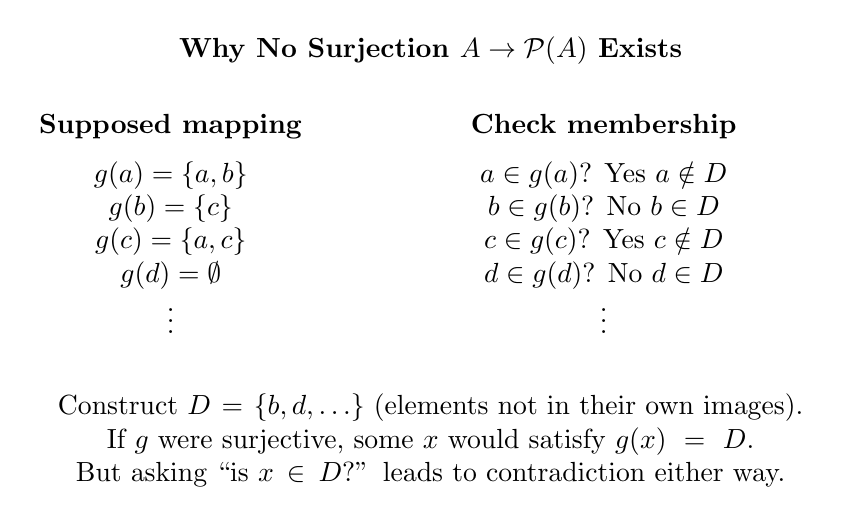
\begin{tikzpicture}[scale=1.1]
    \node at (5, 5) {\textbf{Why No Surjection $A \to \mathcal{P}(A)$ Exists}};
    
    \node[align=center] at (2, 3) {
        \textbf{Supposed mapping} \\[0.2cm]
        $g(a) = \{a, b\}$ \\
        $g(b) = \{c\}$ \\
        $g(c) = \{a, c\}$ \\
        $g(d) = \emptyset$ \\
        $\vdots$
    };
    
    \node[align=center] at (7, 3) {
        \textbf{Check membership} \\[0.2cm]
        $a \in g(a)$? Yes $\implies a \notin D$ \\
        $b \in g(b)$? No $\implies b \in D$ \\
        $c \in g(c)$? Yes $\implies c \notin D$ \\
        $d \in g(d)$? No $\implies d \in D$ \\
        $\vdots$
    };
    
    \node[align=center, text width=10cm] at (5, 0.5) {
        Construct $D = \{b, d, \ldots\}$ (elements not in their own images). \\
        If $g$ were surjective, some $x$ would satisfy $g(x) = D$. \\
        But asking ``is $x \in D$?'' leads to contradiction either way.
    };
\end{tikzpicture}
\end{center}

\begin{warning}
Cantor's theorem is closely related to logical paradoxes:

\textbf{Russell's Paradox} (1901): Let $R = \{x : x \notin x\}$ (the set of all sets that don't contain themselves). Is $R \in R$?

This paradox led to the crisis in foundations of mathematics and the development of axiomatic set theory (ZFC) to avoid such contradictions.

Cantor's diagonal set $D$ uses the same self-referential structure but avoids paradox by working within a fixed set $A$.
\end{warning}

\begin{corollary}[Hierarchy of Infinities]
There is an infinite sequence of strictly increasing cardinalities:
\[|\mathbb{N}| < |\mathcal{P}(\mathbb{N})| < |\mathcal{P}(\mathcal{P}(\mathbb{N}))| < |\mathcal{P}(\mathcal{P}(\mathcal{P}(\mathbb{N})})| < \cdots\]

Equivalently, using aleph notation:
\[\aleph_0 < 2^{\aleph_0} < 2^{2^{\aleph_0}} < \cdots\]

There is no ``largest'' infinity.
\end{corollary}

\section{The Schröder-Bernstein Theorem}

\begin{intuition}
Suppose $|A| \leq |B|$ (injection $A \to B$) and $|B| \leq |A|$ (injection $B \to A$).

Intuitively, this suggests $|A| = |B|$.

But how do we construct a bijection?

The Schröder-Bernstein theorem guarantees one exists.
\end{intuition}

\begin{theorem}[Schröder-Bernstein Theorem]\index{Schroder-Bernstein theorem@Schröder-Bernstein theorem}\index{cardinality!Schroder-Bernstein@Schröder-Bernstein}
If $|A| \leq |B|$ and $|B| \leq |A|$, then $|A| = |B|$.

Equivalently: If there exist injections $f: A \to B$ and $g: B \to A$, then there exists a bijection $h: A \to B$.
\end{theorem}

\begin{proof}[Proof Sketch]
The full proof is intricate, but the idea is:

\begin{enumerate}
    \item Start with injections $f: A \to B$ and $g: B \to A$
    \item Partition $A$ into:
    \begin{itemize}
        \item Elements that ``come from $B$'' (in the image of $g$)
        \item Elements that don't (outside the image of $g$)
    \end{itemize}
    \item Define the bijection $h: A \to B$ by:
    \[h(a) = \begin{cases}
    f(a) & \text{if } a \text{ is not in } \text{Im}(g) \\
    g^{-1}(a) & \text{if } a \text{ is in } \text{Im}(g)
    \end{cases}\]
    \item Verify $h$ is indeed a bijection (uses careful case analysis)
\end{enumerate}

The full rigorous proof requires iterating the injections and using limiting arguments.
\end{proof}

\begin{example}
We can use Schröder-Bernstein to show $|(0, 1)| = |\mathbb{R}|$ without explicit bijection:

\begin{itemize}
    \item Injection $(0, 1) \to \mathbb{R}$: $f(x) = x$ (inclusion)
    \item Injection $\mathbb{R} \to (0, 1)$: $g(x) = \frac{1}{\pi} \arctan(x) + \frac{1}{2}$
\end{itemize}

By Schröder-Bernstein: $|(0, 1)| = |\mathbb{R}|$. $\checkmark$
\end{example}

\section{Cardinal Arithmetic}

\subsection{Addition and Multiplication}

\begin{definition}[Cardinal Arithmetic]
For cardinals $\kappa = |A|$ and $\lambda = |B|$ (where $A \cap B = \emptyset$):

\textbf{Addition}: $\kappa + \lambda = |A \cup B|$ (disjoint union)

\textbf{Multiplication}: $\kappa \cdot \lambda = |A \times B|$ (Cartesian product)

\textbf{Exponentiation}: $\kappa^\lambda = |B^A|$ (set of all functions $A \to B$)
\end{definition}

\begin{theorem}[Arithmetic with $\aleph_0$]
\begin{enumerate}
    \item $\aleph_0 + 1 = \aleph_0$
    \item $\aleph_0 + \aleph_0 = \aleph_0$
    \item $\aleph_0 \cdot \aleph_0 = \aleph_0$
    \item $2^{\aleph_0} = \mathfrak{c} = |\mathbb{R}|$
\end{enumerate}
\end{theorem}

\begin{proof}
\textbf{(1)} $|\mathbb{N}| + 1 = |\mathbb{N} \cup \{*\}|$ where $* \notin \mathbb{N}$.

Bijection: $f(n) = n+1$ for $n \in \mathbb{N}$, $f(*) = 0$. $\checkmark$

\textbf{(2)} $|\mathbb{N}| + |\mathbb{N}| = |\mathbb{N} \cup (\mathbb{N} \times \{1\})|$.

Use the even-odd trick: evens → first copy, odds → second copy. $\checkmark$

\textbf{(3)} We proved $|\mathbb{N} \times \mathbb{N}| = |\mathbb{N}|$ via Cantor pairing. $\checkmark$

\textbf{(4)} We know $|\mathcal{P}(\mathbb{N})| = 2^{\aleph_0}$ (set of all subsets of $\mathbb{N}$).

Each subset corresponds to an infinite binary sequence (characteristic function).

Binary sequences correspond to reals in $(0, 1)$ in binary expansion.

Therefore $2^{\aleph_0} = |\mathcal{P}(\mathbb{N})| = |(0, 1)| = |\mathbb{R}| = \mathfrak{c}$. $\checkmark$
\end{proof}

\subsection{The Continuum Hypothesis}

\begin{keyidea}
We know:
\[\aleph_0 < \mathfrak{c} = 2^{\aleph_0}\]

But are there any cardinalities \textit{between} $\aleph_0$ and $\mathfrak{c}$?
\end{keyidea}

\begin{hypothesis}[Continuum Hypothesis (CH)]
There is no set $S$ with:
\[|\mathbb{N}| < |S| < |\mathbb{R}|\]

Equivalently: $2^{\aleph_0} = \aleph_1$ (the ``next'' infinity after $\aleph_0$).
\end{hypothesis}

\begin{remark}
The continuum hypothesis was Hilbert's first problem in his famous 1900 list.

\textbf{Gödel (1940)}: Proved CH cannot be disproved from ZFC axioms.

\textbf{Cohen (1963)}: Proved CH cannot be proved from ZFC axioms.

\textbf{Conclusion}: CH is \textbf{independent} of ZFC---it's neither true nor false within standard set theory!

You can do mathematics assuming CH is true, or assuming it's false---both are consistent.
\end{remark}

\section{Applications and Implications}

\begin{example}[Almost All Reals are Transcendental]
\textbf{Algebraic numbers}: Roots of polynomials with integer coefficients (e.g., $\sqrt{2}$, $\sqrt[3]{5}$).

\textbf{Transcendental numbers}: Not algebraic (e.g., $\pi$, $e$).

\textbf{Claim}: The algebraic numbers are countable, but the reals are uncountable.

Therefore, ``almost all'' reals are transcendental!

\begin{proof}
Each polynomial $a_n x^n + \cdots + a_1 x + a_0$ with integer coefficients corresponds to a finite tuple $(a_n, \ldots, a_0) \in \mathbb{Z}^{n+1}$.

The set of all such tuples is countable (countable union of countable sets).

Each polynomial has finitely many roots.

Therefore, the set of algebraic numbers is a countable union of finite sets, hence countable.

But $|\mathbb{R}| = \mathfrak{c} > \aleph_0$, so the transcendental numbers are uncountable.
\end{proof}
\end{example}

\begin{example}[Most Functions are Not Computable]
A function $f: \mathbb{N} \to \mathbb{N}$ is \textbf{computable} if there's an algorithm to compute $f(n)$.

\textbf{Claim}: Most functions $\mathbb{N} \to \mathbb{N}$ are not computable.

\begin{proof}
The set of computable functions is countable (each algorithm is a finite string, and there are countably many finite strings).

But $|\mathbb{N}^{\mathbb{N}}| = |\mathbb{N}|^{|\mathbb{N}|} = \aleph_0^{\aleph_0} = \mathfrak{c}$ (uncountable).

Therefore, the set of non-computable functions is uncountable.
\end{proof}

This shows that the computable world is a tiny fraction of the mathematical universe.
\end{example}

\section{Looking Forward}

Cardinality is the foundation for:
\begin{itemize}
    \item \textbf{Measure Theory}: Lebesgue measure, probability spaces
    \item \textbf{Topology}: Separability, compactness, connectedness
    \item \textbf{Computability Theory}: Decidability, Turing machines, complexity
    \item \textbf{Cardinal Arithmetic}: Generalized continuum hypothesis, large cardinals
\end{itemize}

We've seen that infinity comes in many sizes, and that bijections are the key to comparing them.

Next, we embark on one of the most significant constructions in mathematics: rigorously building the \textbf{Real Numbers} from the rationals, finally filling the "gaps" and laying the groundwork for calculus.

\begin{center}
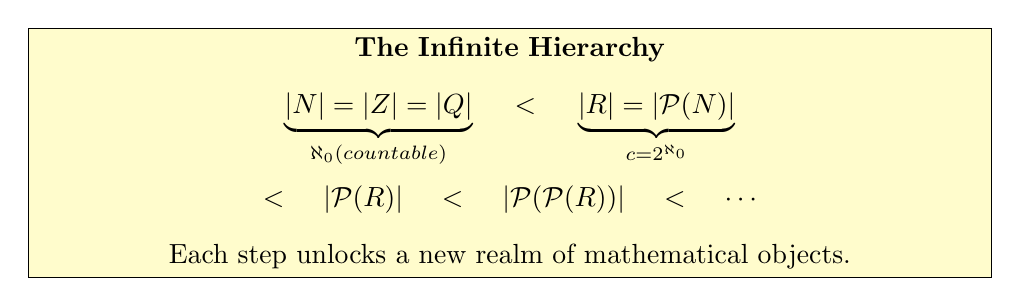
\begin{tikzpicture}[scale=1.0]
    \node[rectangle, draw, fill=yellow!20, text width=12cm, align=center] at (6,0) {
    \textbf{The Infinite Hierarchy} \\[0.3cm]
    $\underbrace{|\mathbb{N}| = |\mathbb{Z}| = |\mathbb{Q}|}_{\aleph_0 \text{ (countable)}} < 
    \underbrace{|\mathbb{R}| = |\mathcal{P}(\mathbb{N})|}_{\mathfrak{c} = 2^{\aleph_0}}$ \\[0.2cm]
    $< |\mathcal{P}(\mathbb{R})| < |\mathcal{P}(\mathcal{P}(\mathbb{R}))| < \cdots$ \\[0.3cm]
    Each step unlocks a new realm of mathematical objects.
    };
\end{tikzpicture}
\end{center}
